\documentclass[10pt, compress]{beamer}
\XeTeXlinebreaklocale "ja"
\XeTeXlinebreakskip=0em plus 0.1em minus 0.01em

\usetheme[usetitleprogressbar]{m}

\usepackage{booktabs}
\usepackage{minted}
\usepackage{fontawesome}
\usepackage{gnuplot-lua-tikz}
\usepackage{tcolorbox}

%%% user macro
\definecolor{links}{HTML}{DB4D6D} % NAKABENI
\hypersetup{colorlinks,linkcolor=,urlcolor=links}

\tcbset{
	width=.9\linewidth
}

\newcommand{\ehref}[2]{\href{#1}{#2 \hspace{-.2em}{\scriptsize\faExternalLink}}}
%\newcommand{\eurl}[1]{\url{#1{\scriptsize \hspace{-.2em}\faExternalLink}}}
%%%

\usepgfplotslibrary{dateplot}

\usemintedstyle{trac}

\title{マルチポート10G NICの試作}
\subtitle{}
%\date{\today}
%\author{Name (\ehref{http://twitter.com/twitter}{\faTwitter  twitter})}
\author{Yohei Kuga@KEIO Univ}
\institute{高速PCルータ研究会 2015/5}

\begin{document}

\maketitle

%% -------------------------------------------------- %%

\begin{frame}[fragile,t]{今日の話}
\begin{itemize}
\item FPGAで合成可能なSystemVerilogによるパケット処理を考える
\item NIC Offload機能の整理
\item Offload拡張機能
\end{itemize}
\end{frame}

%% -------------------------------------------------- %%

\begin{frame}[fragile,t]{その他のNIC実装}
\begin{itemize}
	\item VC709 Connectivity TRD
	\begin{itemize}
		\item 合成時間: 約2h
	\end{itemize}
	\item NetFPGA (NAAS)
\end{itemize}
\end{frame}

%% -------------------------------------------------- %%

\begin{frame}[fragile,t]{今日の話}

ネットワークを高機能化するためにNICを自由に拡張したい
\vspace{.5em}

最近のDC+SW界隈 (Kernel bypass/Unikernels) に比べて,ネットワークHWはまだまだユーザ拡張性が低い
\vspace{-.5em}
\begin{itemize}
\item 現在のOffload機能はL2\~{}L4パケットヘッダ操作が主流
    \begin{itemize}
        \item Capsulation, CSUM, TCP など
    \end{itemize}
\item Programmable NICの検討は始まっている
\end{itemize}
\vspace{.5em}

"NICがProgrammableであること"が最初の一歩
\vspace{-.5em}
\begin{itemize}
\item ヘッダやFIB操作はProgrammable NICやNPUで実現可能
\item ペイロード操作/Interrupt/PCIe/遅延制御などを直接触りたいならFPGA NICが有力
\end{itemize}

\end{frame}

%%%%%%%%%%%%%%%%%%%%%%%

\begin{frame}[fragile,t]
  \frametitle{Systemverilogによるパケット処理例 [1/3]}

\begin{figure}

\begin{minted}[fontsize=\small]{verilog}
union packed {
        bit [5:0][63:0] raw;      // XGMII (64bit)
        struct packed {
                ethhdr eth;
                iphdr ip;
                udphdr udp;
                bit [47:0] payload;
        } hdr;
} tx_pkt, rx_pkt;
\end{minted}
\vspace{-1em}
\caption{パケット構造}
\end{figure}

\end{frame}

%%%%%%%%%%%%%%%%%%%%%%%%%


\begin{frame}[fragile,t]
  \frametitle{Systemverilogによるパケット処理例 [2/3]}

\begin{figure}
\begin{minted}[fontsize=\small]{verilog}
/* MAC adderss */
typedef bit [ETH_ALEN-1:0][7:0] macaddr_t;

/* ethernet header */
typedef struct packed {
        macaddr_t h_dest;
        macaddr_t h_source;
        bit [15:0] h_proto;
} ethhdr;
\end{minted}
\vspace{-1em}
\caption{パケット構造}
\end{figure}

\end{frame}

%%%%%%%%%%%%%%%%%%%%%%%%%

\begin{frame}{マスク(物理)}

\begin{figure}
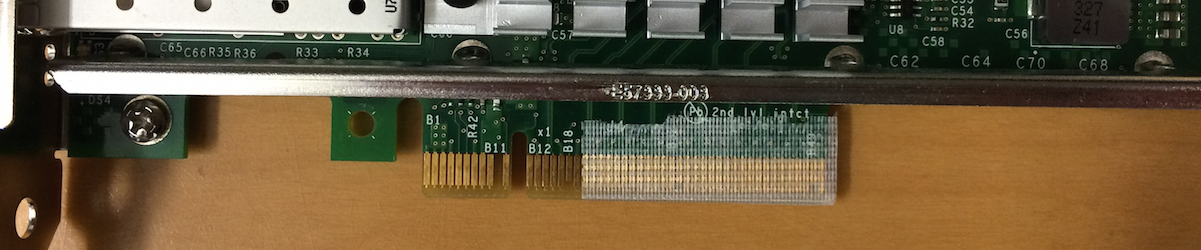
\includegraphics[width=.9\textwidth]{pic/x1.png} \\
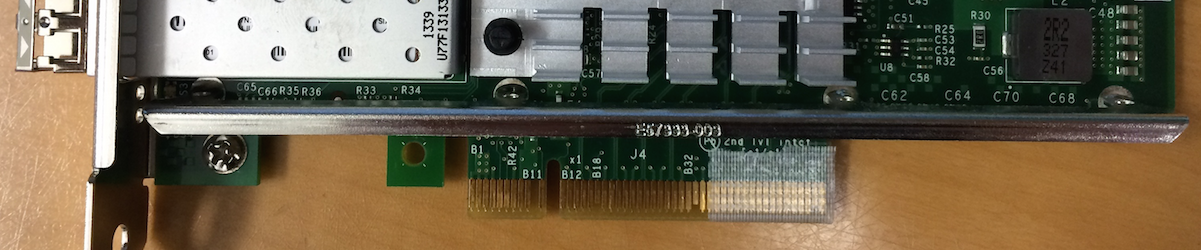
\includegraphics[width=.9\textwidth]{pic/x4.png}

\begin{scriptsize}
\begin{tcolorbox}[]
\$ sudo lspci -vv\\
01:00.0 Ethernet controller: Intel Corporation 82599ES\\
LnkCap: Port \#0, \textbf{Speed 5GT/s, Width x8}, ... \\
LnkSta: \textbf{Speed 5GT/s, Width x1}, ...
\end{tcolorbox}
\end{scriptsize}
\vspace{-.5em}
\small{上: x1マスク, 中: x4マスク, 下: x1時のコンソール}
\end{figure}


\end{frame}

%%%%%%%%%%%%%%%%%%%%%%%%%

\begin{frame}{Throughput for Intel x520 TX}
	\begin{figure}
		\resizebox{.7\textwidth}{!}{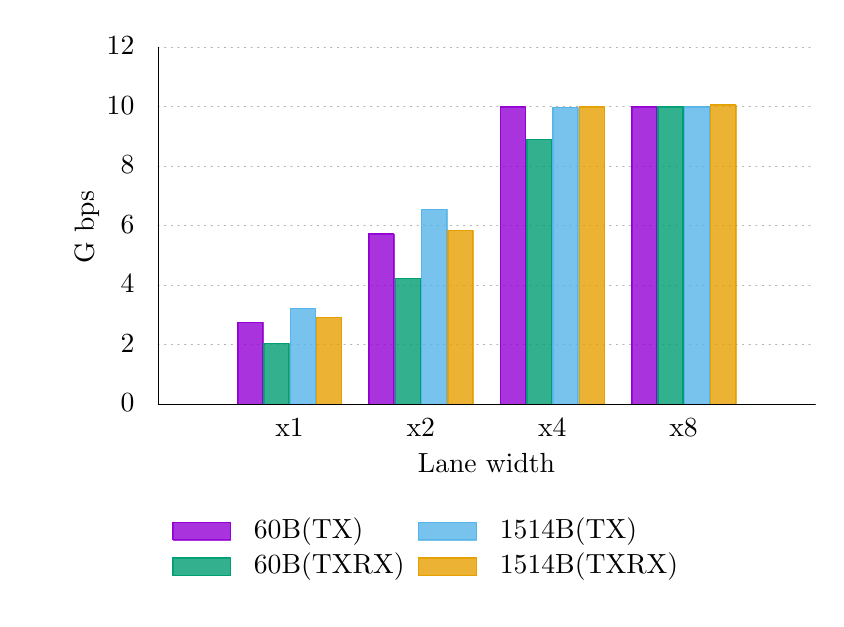
\begin{tikzpicture}[gnuplot]
%% generated with GNUPLOT 5.0p0 (Lua 5.2; terminal rev. 99, script rev. 100)
%% 月  6/29 16:18:40 2015
\path (0.000,0.000) rectangle (10.000,7.000);
\gpcolor{color=gp lt color axes}
\gpsetlinetype{gp lt axes}
\gpsetdashtype{gp dt axes}
\gpsetlinewidth{1.00}
\draw[gp path] (1.656,2.464)--(9.999,2.464);
\gpcolor{color=gp lt color border}
\node[gp node right] at (1.472,2.464) {$0$};
\gpcolor{color=gp lt color axes}
\draw[gp path] (1.656,3.220)--(9.999,3.220);
\gpcolor{color=gp lt color border}
\node[gp node right] at (1.472,3.220) {$2$};
\gpcolor{color=gp lt color axes}
\draw[gp path] (1.656,3.976)--(9.999,3.976);
\gpcolor{color=gp lt color border}
\node[gp node right] at (1.472,3.976) {$4$};
\gpcolor{color=gp lt color axes}
\draw[gp path] (1.656,4.732)--(9.999,4.732);
\gpcolor{color=gp lt color border}
\node[gp node right] at (1.472,4.732) {$6$};
\gpcolor{color=gp lt color axes}
\draw[gp path] (1.656,5.487)--(9.999,5.487);
\gpcolor{color=gp lt color border}
\node[gp node right] at (1.472,5.487) {$8$};
\gpcolor{color=gp lt color axes}
\draw[gp path] (1.656,6.243)--(9.999,6.243);
\gpcolor{color=gp lt color border}
\node[gp node right] at (1.472,6.243) {$10$};
\gpcolor{color=gp lt color axes}
\draw[gp path] (1.656,6.999)--(9.999,6.999);
\gpcolor{color=gp lt color border}
\node[gp node right] at (1.472,6.999) {$12$};
\node[gp node center] at (3.325,2.156) {x1};
\node[gp node center] at (4.993,2.156) {x2};
\node[gp node center] at (6.662,2.156) {x4};
\node[gp node center] at (8.330,2.156) {x8};
\gpsetlinetype{gp lt border}
\gpsetdashtype{gp dt solid}
\draw[gp path] (1.656,6.999)--(1.656,2.464)--(9.999,2.464);
\node[gp node center,rotate=-270] at (0.766,4.731) {G bps};
\node[gp node center] at (5.827,1.694) {Lane width};
\node[gp node left] at (2.756,0.855) {60B(TX)};
\gpfill{rgb color={0.580,0.000,0.827},opacity=0.80} (1.840,0.743)--(2.572,0.743)--(2.572,0.968)--(1.840,0.968)--cycle;
\gpcolor{rgb color={0.580,0.000,0.827}}
\draw[gp path] (1.840,0.743)--(2.572,0.743)--(2.572,0.967)--(1.840,0.967)--cycle;
\gpfill{rgb color={0.580,0.000,0.827},opacity=0.80} (2.666,2.464)--(2.984,2.464)--(2.984,3.511)--(2.666,3.511)--cycle;
\draw[gp path] (2.666,2.464)--(2.666,3.510)--(2.983,3.510)--(2.983,2.464)--cycle;
\gpfill{rgb color={0.580,0.000,0.827},opacity=0.80} (4.334,2.464)--(4.652,2.464)--(4.652,4.633)--(4.334,4.633)--cycle;
\draw[gp path] (4.334,2.464)--(4.334,4.632)--(4.651,4.632)--(4.651,2.464)--cycle;
\gpfill{rgb color={0.580,0.000,0.827},opacity=0.80} (6.003,2.464)--(6.321,2.464)--(6.321,6.244)--(6.003,6.244)--cycle;
\draw[gp path] (6.003,2.464)--(6.003,6.243)--(6.320,6.243)--(6.320,2.464)--cycle;
\gpfill{rgb color={0.580,0.000,0.827},opacity=0.80} (7.671,2.464)--(7.989,2.464)--(7.989,6.244)--(7.671,6.244)--cycle;
\draw[gp path] (7.671,2.464)--(7.671,6.243)--(7.988,6.243)--(7.988,2.464)--cycle;
\gpcolor{color=gp lt color border}
\node[gp node left] at (2.756,0.405) {60B(TXRX)};
\gpfill{rgb color={0.000,0.620,0.451},opacity=0.80} (1.840,0.293)--(2.572,0.293)--(2.572,0.518)--(1.840,0.518)--cycle;
\gpcolor{rgb color={0.000,0.620,0.451}}
\draw[gp path] (1.840,0.293)--(2.572,0.293)--(2.572,0.517)--(1.840,0.517)--cycle;
\gpfill{rgb color={0.000,0.620,0.451},opacity=0.80} (2.999,2.464)--(3.317,2.464)--(3.317,3.238)--(2.999,3.238)--cycle;
\draw[gp path] (2.999,2.464)--(2.999,3.237)--(3.316,3.237)--(3.316,2.464)--cycle;
\gpfill{rgb color={0.000,0.620,0.451},opacity=0.80} (4.668,2.464)--(4.986,2.464)--(4.986,4.069)--(4.668,4.069)--cycle;
\draw[gp path] (4.668,2.464)--(4.668,4.068)--(4.985,4.068)--(4.985,2.464)--cycle;
\gpfill{rgb color={0.000,0.620,0.451},opacity=0.80} (6.336,2.464)--(6.654,2.464)--(6.654,5.833)--(6.336,5.833)--cycle;
\draw[gp path] (6.336,2.464)--(6.336,5.832)--(6.653,5.832)--(6.653,2.464)--cycle;
\gpfill{rgb color={0.000,0.620,0.451},opacity=0.80} (8.005,2.464)--(8.323,2.464)--(8.323,6.244)--(8.005,6.244)--cycle;
\draw[gp path] (8.005,2.464)--(8.005,6.243)--(8.322,6.243)--(8.322,2.464)--cycle;
\gpcolor{color=gp lt color border}
\node[gp node left] at (5.880,0.855) {1514B(TX)};
\gpfill{rgb color={0.337,0.706,0.914},opacity=0.80} (4.964,0.743)--(5.696,0.743)--(5.696,0.968)--(4.964,0.968)--cycle;
\gpcolor{rgb color={0.337,0.706,0.914}}
\draw[gp path] (4.964,0.743)--(5.696,0.743)--(5.696,0.967)--(4.964,0.967)--cycle;
\gpfill{rgb color={0.337,0.706,0.914},opacity=0.80} (3.333,2.464)--(3.651,2.464)--(3.651,3.682)--(3.333,3.682)--cycle;
\draw[gp path] (3.333,2.464)--(3.333,3.681)--(3.650,3.681)--(3.650,2.464)--cycle;
\gpfill{rgb color={0.337,0.706,0.914},opacity=0.80} (5.002,2.464)--(5.320,2.464)--(5.320,4.942)--(5.002,4.942)--cycle;
\draw[gp path] (5.002,2.464)--(5.002,4.941)--(5.319,4.941)--(5.319,2.464)--cycle;
\gpfill{rgb color={0.337,0.706,0.914},opacity=0.80} (6.670,2.464)--(6.988,2.464)--(6.988,6.240)--(6.670,6.240)--cycle;
\draw[gp path] (6.670,2.464)--(6.670,6.239)--(6.987,6.239)--(6.987,2.464)--cycle;
\gpfill{rgb color={0.337,0.706,0.914},opacity=0.80} (8.339,2.464)--(8.657,2.464)--(8.657,6.243)--(8.339,6.243)--cycle;
\draw[gp path] (8.339,2.464)--(8.339,6.242)--(8.656,6.242)--(8.656,2.464)--cycle;
\gpcolor{color=gp lt color border}
\node[gp node left] at (5.880,0.405) {1514B(TXRX)};
\gpfill{rgb color={0.902,0.624,0.000},opacity=0.80} (4.964,0.293)--(5.696,0.293)--(5.696,0.518)--(4.964,0.518)--cycle;
\gpcolor{rgb color={0.902,0.624,0.000}}
\draw[gp path] (4.964,0.293)--(5.696,0.293)--(5.696,0.517)--(4.964,0.517)--cycle;
\gpfill{rgb color={0.902,0.624,0.000},opacity=0.80} (3.667,2.464)--(3.985,2.464)--(3.985,3.569)--(3.667,3.569)--cycle;
\draw[gp path] (3.667,2.464)--(3.667,3.568)--(3.984,3.568)--(3.984,2.464)--cycle;
\gpfill{rgb color={0.902,0.624,0.000},opacity=0.80} (5.335,2.464)--(5.653,2.464)--(5.653,4.679)--(5.335,4.679)--cycle;
\draw[gp path] (5.335,2.464)--(5.335,4.678)--(5.652,4.678)--(5.652,2.464)--cycle;
\gpfill{rgb color={0.902,0.624,0.000},opacity=0.80} (7.004,2.464)--(7.322,2.464)--(7.322,6.245)--(7.004,6.245)--cycle;
\draw[gp path] (7.004,2.464)--(7.004,6.244)--(7.321,6.244)--(7.321,2.464)--cycle;
\gpfill{rgb color={0.902,0.624,0.000},opacity=0.80} (8.672,2.464)--(8.990,2.464)--(8.990,6.269)--(8.672,6.269)--cycle;
\draw[gp path] (8.672,2.464)--(8.672,6.268)--(8.989,6.268)--(8.989,2.464)--cycle;
\gpcolor{color=gp lt color border}
\draw[gp path] (1.656,6.999)--(1.656,2.464)--(9.999,2.464);
%% coordinates of the plot area
\gpdefrectangularnode{gp plot 1}{\pgfpoint{1.656cm}{2.464cm}}{\pgfpoint{9.999cm}{6.999cm}}
\end{tikzpicture}
%% gnuplot variables
}
	\end{figure}
	{\footnotesize Theoretical Max. Throughput (PCIe gen2): \\ x1: 5GT/s, x2: 10GT/s, x4: 20GT/s, x8: 40GT/s}
\end{frame}

%%%%%%%%%%%%%%%%%%%%%%%%%

\begin{frame}{\% of Theoretical Maximum Throughput for Intel x520 TX}
	\begin{figure}
		\resizebox{.7\textwidth}{!}{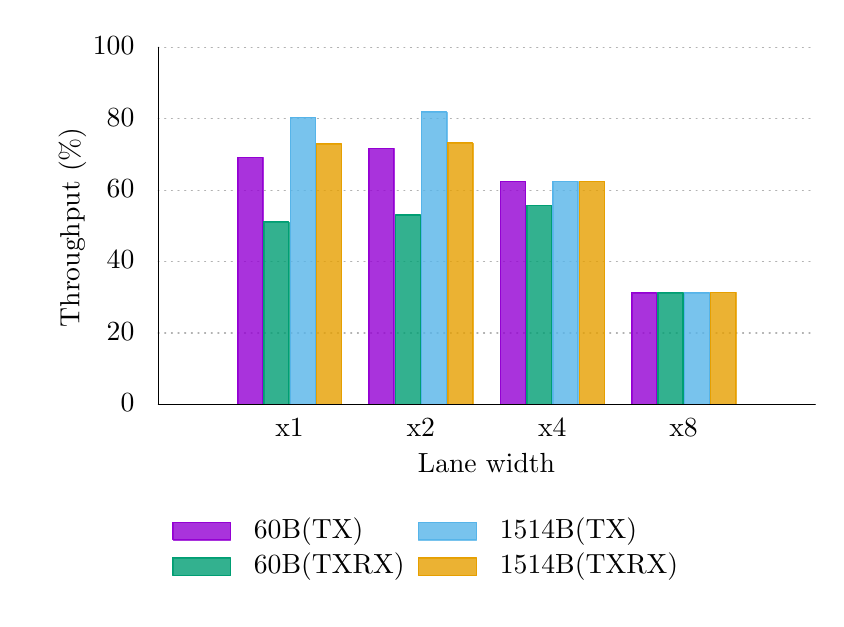
\begin{tikzpicture}[gnuplot]
%% generated with GNUPLOT 5.0p0 (Lua 5.2; terminal rev. 99, script rev. 100)
%% 金  5/ 8 21:37:03 2015
\path (0.000,0.000) rectangle (10.000,7.000);
\gpcolor{color=gp lt color axes}
\gpsetlinetype{gp lt axes}
\gpsetdashtype{gp dt axes}
\gpsetlinewidth{1.00}
\draw[gp path] (1.656,2.464)--(9.999,2.464);
\gpcolor{color=gp lt color border}
\node[gp node right] at (1.472,2.464) {$0$};
\gpcolor{color=gp lt color axes}
\draw[gp path] (1.656,3.371)--(9.999,3.371);
\gpcolor{color=gp lt color border}
\node[gp node right] at (1.472,3.371) {$20$};
\gpcolor{color=gp lt color axes}
\draw[gp path] (1.656,4.278)--(9.999,4.278);
\gpcolor{color=gp lt color border}
\node[gp node right] at (1.472,4.278) {$40$};
\gpcolor{color=gp lt color axes}
\draw[gp path] (1.656,5.185)--(9.999,5.185);
\gpcolor{color=gp lt color border}
\node[gp node right] at (1.472,5.185) {$60$};
\gpcolor{color=gp lt color axes}
\draw[gp path] (1.656,6.092)--(9.999,6.092);
\gpcolor{color=gp lt color border}
\node[gp node right] at (1.472,6.092) {$80$};
\gpcolor{color=gp lt color axes}
\draw[gp path] (1.656,6.999)--(9.999,6.999);
\gpcolor{color=gp lt color border}
\node[gp node right] at (1.472,6.999) {$100$};
\node[gp node center] at (3.325,2.156) {x1};
\node[gp node center] at (4.993,2.156) {x2};
\node[gp node center] at (6.662,2.156) {x4};
\node[gp node center] at (8.330,2.156) {x8};
\gpsetlinetype{gp lt border}
\gpsetdashtype{gp dt solid}
\draw[gp path] (1.656,6.999)--(1.656,2.464)--(9.999,2.464);
\node[gp node center,rotate=-270] at (0.582,4.731) {Throughput (\%)};
\node[gp node center] at (5.827,1.694) {Lane width};
\node[gp node left] at (2.756,0.855) {60B(TX)};
\gpfill{rgb color={0.580,0.000,0.827},opacity=0.80} (1.840,0.743)--(2.572,0.743)--(2.572,0.968)--(1.840,0.968)--cycle;
\gpcolor{rgb color={0.580,0.000,0.827}}
\draw[gp path] (1.840,0.743)--(2.572,0.743)--(2.572,0.967)--(1.840,0.967)--cycle;
\gpfill{rgb color={0.580,0.000,0.827},opacity=0.80} (2.666,2.464)--(2.984,2.464)--(2.984,5.605)--(2.666,5.605)--cycle;
\draw[gp path] (2.666,2.464)--(2.666,5.604)--(2.983,5.604)--(2.983,2.464)--cycle;
\gpfill{rgb color={0.580,0.000,0.827},opacity=0.80} (4.334,2.464)--(4.652,2.464)--(4.652,5.718)--(4.334,5.718)--cycle;
\draw[gp path] (4.334,2.464)--(4.334,5.717)--(4.651,5.717)--(4.651,2.464)--cycle;
\gpfill{rgb color={0.580,0.000,0.827},opacity=0.80} (6.003,2.464)--(6.321,2.464)--(6.321,5.299)--(6.003,5.299)--cycle;
\draw[gp path] (6.003,2.464)--(6.003,5.298)--(6.320,5.298)--(6.320,2.464)--cycle;
\gpfill{rgb color={0.580,0.000,0.827},opacity=0.80} (7.671,2.464)--(7.989,2.464)--(7.989,3.882)--(7.671,3.882)--cycle;
\draw[gp path] (7.671,2.464)--(7.671,3.881)--(7.988,3.881)--(7.988,2.464)--cycle;
\gpcolor{color=gp lt color border}
\node[gp node left] at (2.756,0.405) {60B(TXRX)};
\gpfill{rgb color={0.000,0.620,0.451},opacity=0.80} (1.840,0.293)--(2.572,0.293)--(2.572,0.518)--(1.840,0.518)--cycle;
\gpcolor{rgb color={0.000,0.620,0.451}}
\draw[gp path] (1.840,0.293)--(2.572,0.293)--(2.572,0.517)--(1.840,0.517)--cycle;
\gpfill{rgb color={0.000,0.620,0.451},opacity=0.80} (2.999,2.464)--(3.317,2.464)--(3.317,4.784)--(2.999,4.784)--cycle;
\draw[gp path] (2.999,2.464)--(2.999,4.783)--(3.316,4.783)--(3.316,2.464)--cycle;
\gpfill{rgb color={0.000,0.620,0.451},opacity=0.80} (4.668,2.464)--(4.986,2.464)--(4.986,4.871)--(4.668,4.871)--cycle;
\draw[gp path] (4.668,2.464)--(4.668,4.870)--(4.985,4.870)--(4.985,2.464)--cycle;
\gpfill{rgb color={0.000,0.620,0.451},opacity=0.80} (6.336,2.464)--(6.654,2.464)--(6.654,4.991)--(6.336,4.991)--cycle;
\draw[gp path] (6.336,2.464)--(6.336,4.990)--(6.653,4.990)--(6.653,2.464)--cycle;
\gpfill{rgb color={0.000,0.620,0.451},opacity=0.80} (8.005,2.464)--(8.323,2.464)--(8.323,3.882)--(8.005,3.882)--cycle;
\draw[gp path] (8.005,2.464)--(8.005,3.881)--(8.322,3.881)--(8.322,2.464)--cycle;
\gpcolor{color=gp lt color border}
\node[gp node left] at (5.880,0.855) {1514B(TX)};
\gpfill{rgb color={0.337,0.706,0.914},opacity=0.80} (4.964,0.743)--(5.696,0.743)--(5.696,0.968)--(4.964,0.968)--cycle;
\gpcolor{rgb color={0.337,0.706,0.914}}
\draw[gp path] (4.964,0.743)--(5.696,0.743)--(5.696,0.967)--(4.964,0.967)--cycle;
\gpfill{rgb color={0.337,0.706,0.914},opacity=0.80} (3.333,2.464)--(3.651,2.464)--(3.651,6.114)--(3.333,6.114)--cycle;
\draw[gp path] (3.333,2.464)--(3.333,6.113)--(3.650,6.113)--(3.650,2.464)--cycle;
\gpfill{rgb color={0.337,0.706,0.914},opacity=0.80} (5.002,2.464)--(5.320,2.464)--(5.320,6.181)--(5.002,6.181)--cycle;
\draw[gp path] (5.002,2.464)--(5.002,6.180)--(5.319,6.180)--(5.319,2.464)--cycle;
\gpfill{rgb color={0.337,0.706,0.914},opacity=0.80} (6.670,2.464)--(6.988,2.464)--(6.988,5.296)--(6.670,5.296)--cycle;
\draw[gp path] (6.670,2.464)--(6.670,5.295)--(6.987,5.295)--(6.987,2.464)--cycle;
\gpfill{rgb color={0.337,0.706,0.914},opacity=0.80} (8.339,2.464)--(8.657,2.464)--(8.657,3.882)--(8.339,3.882)--cycle;
\draw[gp path] (8.339,2.464)--(8.339,3.881)--(8.656,3.881)--(8.656,2.464)--cycle;
\gpcolor{color=gp lt color border}
\node[gp node left] at (5.880,0.405) {1514B(TXRX)};
\gpfill{rgb color={0.902,0.624,0.000},opacity=0.80} (4.964,0.293)--(5.696,0.293)--(5.696,0.518)--(4.964,0.518)--cycle;
\gpcolor{rgb color={0.902,0.624,0.000}}
\draw[gp path] (4.964,0.293)--(5.696,0.293)--(5.696,0.517)--(4.964,0.517)--cycle;
\gpfill{rgb color={0.902,0.624,0.000},opacity=0.80} (3.667,2.464)--(3.985,2.464)--(3.985,5.776)--(3.667,5.776)--cycle;
\draw[gp path] (3.667,2.464)--(3.667,5.775)--(3.984,5.775)--(3.984,2.464)--cycle;
\gpfill{rgb color={0.902,0.624,0.000},opacity=0.80} (5.335,2.464)--(5.653,2.464)--(5.653,5.787)--(5.335,5.787)--cycle;
\draw[gp path] (5.335,2.464)--(5.335,5.786)--(5.652,5.786)--(5.652,2.464)--cycle;
\gpfill{rgb color={0.902,0.624,0.000},opacity=0.80} (7.004,2.464)--(7.322,2.464)--(7.322,5.300)--(7.004,5.300)--cycle;
\draw[gp path] (7.004,2.464)--(7.004,5.299)--(7.321,5.299)--(7.321,2.464)--cycle;
\gpfill{rgb color={0.902,0.624,0.000},opacity=0.80} (8.672,2.464)--(8.990,2.464)--(8.990,3.891)--(8.672,3.891)--cycle;
\draw[gp path] (8.672,2.464)--(8.672,3.890)--(8.989,3.890)--(8.989,2.464)--cycle;
\gpcolor{color=gp lt color border}
\draw[gp path] (1.656,6.999)--(1.656,2.464)--(9.999,2.464);
%% coordinates of the plot area
\gpdefrectangularnode{gp plot 1}{\pgfpoint{1.656cm}{2.464cm}}{\pgfpoint{9.999cm}{6.999cm}}
\end{tikzpicture}
%% gnuplot variables
}
	\end{figure}
	{\footnotesize Theoretical Max. Throughput (PCIe gen2): \\ x1: 5GT/s, x2: 10GT/s, x4: 20GT/s, x8: 40GT/s}
\end{frame}


%%%%%%%%%%%%%%%%%%%%%%%%%

\begin{frame}[fragile]
  \frametitle{mtheme}

  The \emph{mtheme} is a Beamer theme with minimal visual noise inspired by the
  \ehref{https://github.com/hsrmbeamertheme/hsrmbeamertheme}{\textsc{hsrm} Beamer
  Theme} by Benjamin Weiss.

  Enable the theme by loading \faFrown

  \begin{minted}[fontsize=\small]{latex}
    \documentclass{beamer}
    \usetheme{m}
  \end{minted}

  Note, that you have to have Mozilla's \emph{Fira Sans} font and XeTeX
  installed to enjoy this wonderful typography.
\end{frame}

\begin{frame}[fragile]
  \frametitle{Sections}
  Sections group slides of the same topic

  \begin{minted}[fontsize=\small]{latex}
    \section{Elements}
  \end{minted}

  for which the \emph{mtheme} provides a nice progress indicator \ldots
\end{frame}

\section{Elements}

\begin{frame}[fragile]
  \frametitle{Typography}
      \begin{minted}[fontsize=\small]{latex}
The theme provides sensible defaults to \emph{emphasize}
text, \alert{accent} parts or show \textbf{bold} results.
      \end{minted}

  \begin{center}becomes\end{center}

  The theme provides sensible defaults to \emph{emphasize} text,
  \alert{accent} parts or show \textbf{bold} results.
\end{frame}
\begin{frame}{Lists}
  \begin{columns}[onlytextwidth]
    \column{0.5\textwidth}
      Items
      \begin{itemize}
        \item Milk \item Eggs \item Potatos
      \end{itemize}

    \column{0.5\textwidth}
      Enumerations
      \begin{enumerate}
        \item First, \item Second and \item Last.
      \end{enumerate}
  \end{columns}
\end{frame}
\begin{frame}{Descriptions}
  \begin{description}
    \item[PowerPoint] Meeh.
    \item[Beamer] Yeeeha.
  \end{description}
\end{frame}
\begin{frame}{Animation}
  \begin{itemize}[<+- | alert@+>]
    \item \alert<4>{This is\only<4>{ really} important}
    \item Now this
    \item And now this
  \end{itemize}
\end{frame}
\begin{frame}{Figures}
  \begin{figure}
    \newcounter{density}
    \setcounter{density}{20}
    \begin{tikzpicture}
	\def\couleur{mLightBrown}
		\path[coordinate] (0,0)  coordinate(A)
			++( 90:5cm) coordinate(B)
			++(0:5cm) coordinate(C)
			++(-90:5cm) coordinate(D);
		\draw[fill=\couleur!\thedensity] (A) -- (B) -- (C) --(D) -- cycle;
		\foreach \x in {1,...,40}{%
		\pgfmathsetcounter{density}{\thedensity+20}
		\setcounter{density}{\thedensity}
		\path[coordinate] coordinate(X) at (A){};
		\path[coordinate] (A) -- (B) coordinate[pos=.10](A)
			-- (C) coordinate[pos=.10](B)
			-- (D) coordinate[pos=.10](C)
			-- (X) coordinate[pos=.10](D);
		\draw[fill=\couleur!\thedensity] (A)--(B)--(C)-- (D) -- cycle;
		}
\end{tikzpicture}

    \caption{Rotated square from
    \ehref{http://www.texample.net/tikz/examples/rotated-polygons/}{texample.net}.}
  \end{figure}
\end{frame}
\begin{frame}{Tables}
  \begin{table}
    \caption{Largest cities in the world (source: Wikipedia)}
    \begin{tabular}{lr}
      \toprule
      City & Population\\
      \midrule
      Mexico City & 20,116,842\\
      Shanghai & 19,210,000\\
      Peking & 15,796,450\\
      Istanbul & 14,160,467\\
      \bottomrule
    \end{tabular}
  \end{table}
\end{frame}
\begin{frame}{Blocks}

  \begin{block}{This is a block title}
    This is soothing.
  \end{block}

\end{frame}
\begin{frame}{Math}
  \begin{equation*}
    e = \lim_{n\to \infty} \left(1 + \frac{1}{n}\right)^n
  \end{equation*}
\end{frame}
\begin{frame}{Line plots}
  \begin{figure}
    \begin{tikzpicture}
	\begin{axis}[
		mlineplot,
		width=0.9\textwidth,
		height=6cm,
	]

	\addplot {sin(deg(x))};
	\addplot+[samples=100] {sin(deg(2*x))};

	\end{axis}
\end{tikzpicture}

  \end{figure}
\end{frame}
\begin{frame}{Bar charts}
  \begin{figure}
    \begin{tikzpicture}
	\begin{axis}[
		mbarplot,
		xlabel={Foo},
		ylabel={Bar},
		width=0.9\textwidth,
		height=6cm,
	]

	\addplot plot coordinates {(1, 20) (2, 25) (3, 22.4) (4, 12.4)};
	\addplot plot coordinates {(1, 18) (2, 24) (3, 23.5) (4, 13.2)};
	\addplot plot coordinates {(1, 10) (2, 19) (3, 25) (4, 15.2)};

	\legend{lorem, ipsum, dolor}

	\end{axis}
\end{tikzpicture}

  \end{figure}
\end{frame}
\begin{frame}{Quotes}
  \begin{quote}
    Veni, Vidi, Vici
  \end{quote}
\end{frame}


\section{Conclusion}

\begin{frame}{Summary}

  Get the source of this theme and the demo presentation from

  \begin{center}\url{github.com/matze/mtheme}\end{center}

  The theme \emph{itself} is licensed under a
  \ehref{http://creativecommons.org/licenses/by-sa/4.0/}{Creative Commons
  Attribution-ShareAlike 4.0 International License}.

\end{frame}

\plain{Questions? \faSmile}

\end{document}
